\section{Materials and methods}\label{methodology}
\todo{Interest rate des Landlords corresponds zum Mieterwechsel}
This section explains the methodology and the optimization model developed in this work. The section starts with an introduction and overview of the model in Section \ref{met:intro}, followed by a detailed description of the mathematical formulation in Section \ref{met:formulas}. The case study and scenario description is given in Section \ref{met:empirical}. The model validation is described in Section \ref{met:validate} and the open-source programming environment in Section \ref{met:os}

\subsection{Introduction and model overview}\label{met:intro}
This section provides an comprehensive overview of the proposed model. In general, three agents with the following characteristics are considered:
\paragraph{Governance} The governance's main objective is to decarbonizing the residential heating sector. Therefore, the intention is to trigger a heating system change to a sustainable alternative on the multi-apartment building level by financial support for both landlord and tenants. The avowed aim is to find a cost-minimal and socially balanced solution. The financial support can be realized by an investment grant (paid directly from the governance) or rent-charge-related revenues (from the tenants and refunded by the governance) for the landlord and heating costs subsidy payments for the tenants. 
\paragraph{Landlord} is the owner of the multi-apartment building and provides the heating system for the tenants, and is profit-oriented. Thus, a heating system change toward a sustainable alternative only is realized in case of the economic viability of the investment. In this context, the landlord can achieve profitability of the alternative heating system by receiving an investment grant (to reduce the overnight investment costs from the governance) and a rent-charge-related revenue cash flow (from the tenants). 
\paragraph{Tenant} rents a dwelling within the multi-apartment building from the landlord and has rent-related and energy-related spendings. He cannot change the heating system on his authority but depends on the landlord's willingness to realize a low-emission sustainable alternative. Especially in the case of the existing heating system, its costs are directly subject to a higher pricing of CO\textsubscript{2} emissions. Nevertheless, the tenant aims to limit total costs in case of a heating system change at the level of the initial condition.\vspace{0.5cm}

Figure \ref{fig:methodology} shows a sketch illustrating the interrelations between the governance, the landlord, and the tenants. The governance can support the landlord financially by investment grants and by the allowance of rent charge adjustments. At the same time, tenants are supported by a heating costs subsidy payment. The gray bar in the middle indicates that these financial benefits need to be socially balanced and overcome the differences in ownership within the multi-apartment building. The rent or rent charge adjustment is the direct financial exchange between the landlord and the tenant.\vspace{0.5cm}

\begin{figure}[h]
	\centering
	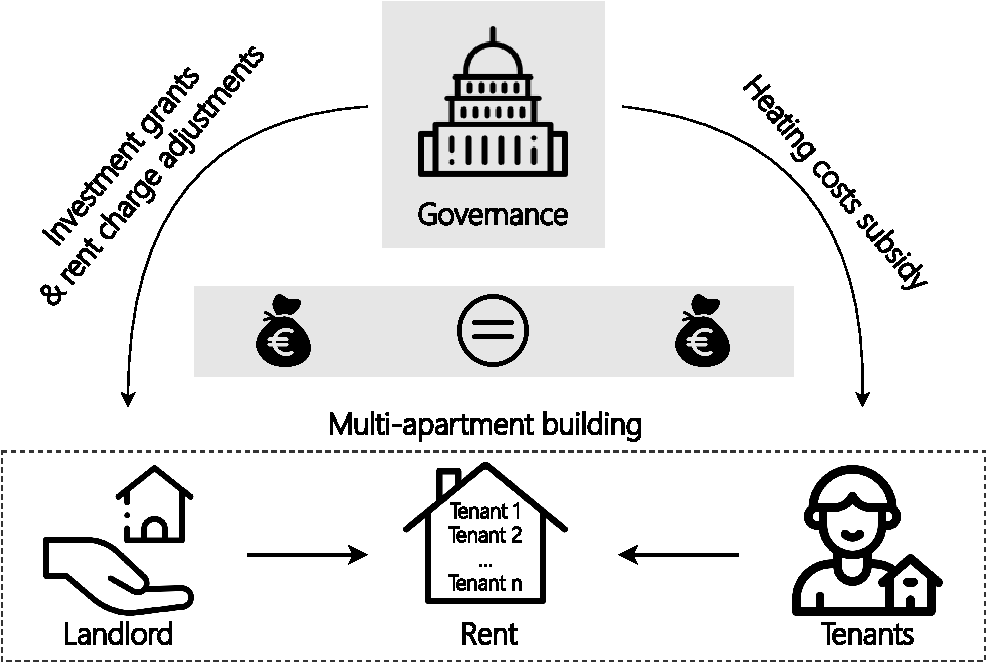
\includegraphics[width=1\linewidth]{figures/3_Methodology/Sketch.pdf}
	\caption{Sketch of the model illustrating the iterrelations between the governance, landlord, and tenants. Financial support from the governance is socially balanced at the multi-apartment building.}
	\label{fig:methodology}
\end{figure}

\subsection{Mathematical formulation of the model}\label{met:formulas}
This section explains the mathematical formulation of the optimization model in detail. First, the objective function is defined. Then, a detailed explanation of the model's constraints is given. 

\subsubsection{Model's objective function}
The objective function of the model is to minimize governance's total costs, including investment grants and subsidy payments\footnote{This corresponds to the maximization of the governance's net present value.}. Therefore, the objective function can be written as follows: 
\begin{align}\label{objective}
\underset{x}{\mathrm{min~}} \Psi + \sum_{y} \sum_{m} \frac{n}{(1+i_g)^y} \cdot \Omega_{y,m}
\end{align}

where $\Psi$ is the investment grant paid to the landlord and $\Omega_{y,m}$ the heating costs subsidy payment paid to a single tenant in year $y$ and month $m$. In addition, $n$ is the number of tenants\footnote{It is assumed that the multi-apartment building consists of $n$ equal tenants.} and $i_g$ the governance's interest rate. The model's decision variables are included in the decision variable vector $x$. We refer to the nomenclature at the beginning of the paper containing a list of all decision variables.

\subsubsection{Model's constraints}
Equation \ref{c:demand} describes the load satisfaction of the total heat demand within the multi-apartment building using the alternative heating system in each time step (year and month) 
\begin{align}\label{c:demand}
n \cdot d_{y,m} \leq q_{y,m} \quad :\forall y,m
\end{align}

where $d_{y,m}$ is the total heat demand of a tenant's dwelling and $q_{y,m}$ the heat demand covered by the alternative heating system in $y$ and $m$. Building on this, Equation \ref{c:capacity} defines the minimum required newly installed capacity of the heating system alternative
\begin{align}\label{c:capacity}
\alpha_{m} \cdot q_{y,m} \leq \pi \quad :\forall y,m
\end{align}

where $\alpha_{m}$ is the load factor transforming the monthly amount of heat demand to the corresponding peak demand. Equation \ref{c:investment} defines the landlord's overnight investment costs ($\zeta$)
\begin{align}\label{c:investment}
\zeta = \pi \cdot c_{alt} + n \cdot c_{con} - \Psi
\end{align}

where $c_{alt}$ is the specific investment costs of the heating system alternative and $c_{con}$ the construction costs of an dwelling. Equation \ref{c:upper_inv_limit} defines the upper bound for the investment grant 
\begin{align}\label{c:upper_inv_limit}
\Psi \leq \hat{d} \cdot c_{alt} + n \cdot c_{con}
\end{align}

where $\hat{d}$ is the peak value of the heat demand. Equation \ref{c:revenues} defines the rent-related revenues of the landlord ($\lambda_{y,m}$)
\begin{align}\label{c:revenues}
\lambda_{y,m} = a \cdot n \cdot (\bar{r} + r_{y,m}) \quad :\forall y,m
\end{align}

where $\bar{r}$ is the initial rent price, $r_{y,m}$ the rent charge adjustment associated with the heating system change in $y$ and $m$ and $a$ the area of a tenant's dwelling. Equation \ref{c:npv} sets the landlord's net present value of the alternative heating system investment equal to zero
\begin{align}\label{c:npv}
-\zeta + \sum_{y} \sum_{m} \frac{1}{(1+i_l)^y} \cdot \lambda_{y,m} = 0
\end{align}

where $i_l$ is the landlord's interest rate. Equation \ref{c:ten1} defines the initial annual spendings of all tenants ($\kappa_{y}$) using the existing heating system 
\begin{align}\label{c:ten1}
\kappa_{y} = n \cdot (\bar{r} \cdot a + \sum_{m} q_{load,y,m} \cdot p_{init,y,m}) \quad :y=y_0
\end{align}

where $p_{init,y,m}$ is the price of the conventional fuel initially supplying the heat demand in $y$ and $m$. Building on this, Equation \ref{c:ten2} sets the tenants' total spendings ($K_{init}$)
\begin{align}\label{c:ten2}
K_{init} = -\sum_{y} \frac{1}{(1+i_{t})^y} \cdot \kappa_{y_0}
\end{align}

where $\sigma_{y_0}$ represents the initial tenants' spendings from Equation \ref{c:ten1} above and $i_t$ the tenant's interest rate. Equation \ref{c:ten3} defines the total spendings of all tenants ($K_{alt}$) realizing the sustainable heating system alternative
\begin{align}\label{c:ten3}
	K_{alt} = -\sum_{y} \sum_{m} \frac{n}{(1+i_{t})^y} \left(a \cdot (\bar{r} + r_{y,m}) + q_{y,m} \cdot p_{alt,y,m}-\Omega_{y,m} \right)
\end{align}

and Equation \ref{c:ten4} defines constant remaining spendings (i.e., economic viability) for the tenants in case of the heating system change.
\begin{align}\label{c:ten4}
K_{alt} = K_{init}
\end{align}

Equation \ref{c:con_sub} defines constant heat costs subsidy payments and Equation \ref{c:con_rent} constant total rent price for a tenant in $y$.
\begin{alignat}{2}
\Omega_{y,m} = \Omega_{y,m-1} \quad &:y\label{c:con_sub}\\
\bar{r} + r_{y,m} = \bar{r} + r_{y,m-1} \quad &:y\label{c:con_rent}
\end{alignat}

Equation \ref{c:temp_rent} allows rent charge adjustment by the landlord only every two years and Equation \ref{c:rent_upper1} and \ref{c:rent_upper2} set a upper bound to the rent charge adjustment
\begin{alignat}{3}
\bar{r} + r_{y,m} = \bar{r} + r_{y-1,m} \quad &:\forall y\backslash \{y_0\},m~\text{if}~y~\text{mod}~2=0\label{c:temp_rent}\\
\bar{r}+r_{y,m} \leq \rho \cdot \bar{r} \quad &:\forall y \in {y_0}\label{c:rent_upper1}\\
\bar{r}+r_{y,m} \leq \rho \cdot \left(\bar{r}+r_{y-1,m}\right) \quad &:\forall y\backslash \{y_0\}\label{c:rent_upper2}
\end{alignat}

by introducing $\rho$, as the rent charge adjustment upper bound. Equation \ref{c:final} defines the financial support parity between the landlord and all tenants at the multi-apartment building level from the governance's perspective 
\begin{align}\label{c:final}
\underbrace{\Psi +  n \cdot \sum_{y} \sum_{m} \frac{r_{y,m}}{(1+i_{g})^y}}_{\text{landlord's financial support}}= \underbrace{n \cdot \sum_{y} \sum_{m} \frac{\Omega_{y,m}}{(1+i_{g})^y}}_{\text{tenants' financial support}}
\end{align}

\subsection{Definition of the case study, scenarios and empirical settings}\label{met:empirical}
\subsubsection{Multi-apartment building}
The model proposed in this paper is applied to a typical multi-apartment building in an urban area. In particular, a partially renovated and natural gas-based heated old building in Vienna, Austria is investigated. In $2020$, there were over \SI{440000}{} natural gas-based heated dwellings in Vienna, Austria (\SI{48.5}{\%} of the total building stock) \cite{statistikaustriaheizen}. Nevertheless, this case study is representative for the European building stock in densely populated areas, as similar proportions of natural gas heating systems exist in the heating sector there as well\footnote{For example, there are more than \SI{600000}{} natural gas-based heat dwellings in Berlin, Germany in $2020$ \cite{BDEW2019}.}.\vspace{0.5cm}

It is assumed that the multi-apartment building (incl. all dwellings) are privately owned by the landlord. The number of dwellings is $30$, whereby the area and rent price for each is equal. Each dwelling is rented by a tenant and heated by a individual natural gas-based heating system. The decarbonization of the heating systems can be realized by two different options, namely, a connection to the district heating network and a installation of a air-sourced heat pump\footnote{In general, it is assumed that the heat pump can be installed in the basement of the building. Nevertheless, the installation on the rooftop may also be considered. However, this explicit distinction is out of the scope of this paper and is not further examined.}. It is assumed, that only of the two options is realized for all the dwellings. We refer to the empirical scaling and data in Section \ref{sec:data} for a detailed quantitative description of the multi-apartment building. 

\subsubsection{Scenarios}
Four different quantitative scenarios are studied in this work. Three of them are developed in the Horizon $2020$ research project openENTRANCE (\url{https://openentrance.eu/}) and describe a future European energy system development under achieving the \SI{1.5}{\degreeCelsius} or \SI{2.0}{\degreeCelsius} climate target. These scenarios are called \textit{Directed Transition}, \textit{Societal Commitment}, and \textit{Gradual Development} scenario\footnote{The openENTRANCE scenario \textit{Techno-Friendly} is not part of this work.}. The first two scenarios consider the remaining CO\textsubscript{2} budget of the \SI{1.5}{\degreeCelsius} climate target. Below, we qualitatively describe the three openENTRANCE scenarios used in this work and refer for further information to the studies in \cite{auer2020development} and \cite{auer2020quantitative}. For the reader with a particular interest in the openENTRANCE scenarios, we refer to the work in \cite{auer2019quantitative}, in which the underlying storylines outlining the narrative frames
of the quantitative scenarios can be found.\vspace{0.5cm}

The \textit{Directed Transition} (DT) scenarios leads to limiting the global temperature increase well below \SI{1.5}{\degreeCelsius}. This is achieved by a breakthrough of new sustainable technologies triggered through strong policy incentives. The markets themselves do not push this development and only deliver insufficient financial impulse for the clean energy transition. Besides, society is also too passive in supporting the penetration of renewable energy sources. Thus, it is assumed that multi-apartment building is connected to the district heating network. The CO\text{2} price is between \SI{196}{EUR \per tCO_{2}} (in 2025) and \SI{680}{EUR \per tCO_{2}} (in 2040). Deep decarbonization of the European electricity and heating sector is achieved in $2040$.\vspace{0.5cm}

The \textit{Societal Commitment} (SC) scenario also leads to limiting the global temperature increase well below \SI{1.5}{\degreeCelsius}. In contrast to the previous scenario, decentralization of the energy system and participatory as well as societal acceptance of energy transition pushes the sustainable development. In addition, currently existing technologies significantly driven by policy incentives contribute to a decarbonized energy system since no fundamental breakthroughs of new clean technologies are in sight. Therefore, the multi-apartment building implements an air-source heat pump as sustainable heating system alternative. The CO\text{2} price in this scenario is between \SI{62}{EUR \per tCO_{2}} (in 2025) and \SI{497}{EUR \per tCO_{2}} (in 2040). Deep decarbonization of the European electricity and heating sector is achieved in $2040$.\vspace{0.5cm}

The \textit{Gradual Development} (GD) scenario reaches a global temperature increase of \SI{2.0}{\degreeCelsius} and the corresponding climate target. In general, it is a very conservative expression of an European energy system future. This scenario includes a little of each sustainable development consisting of limited policy incentives, social acceptance, and technological advances. Both heating system alternatives (district heating connection and air-sourced heat pump installation) are examined. The CO\text{2} price in this scenario is between \SI{83}{EUR \per tCO_{2}} (in 2025) and \SI{261}{EUR \per tCO_{2}} (in 2040). Deep decarbonization of the European electricity and heating sector is achieved in $2050$.\vspace{0.5cm}

In addition to the three openENTRANCE scenarios, the so-called "Low CO\textsubscript{2} price development" (LP) scenario is examined. This scenario neglects any remaining European CO\textsubscript{2} budget and misses both the  \SI{1.5}{\degreeCelsius} and \SI{2.0}{\degreeCelsius} climate target. Thus, decarbonizing the electricity and heating sector develops only sluggishly. Therefore, neither the CO\textsubscript{2} price nor the specific emissions of electricity and district heating significantly significantly changed compared to today's values. Again, both heating system alternatives are studied. The CO\text{2} price in this scenario is between \SI{60}{EUR \per tCO_{2}} (in 2025) and \SI{90}{EUR \per tCO_{2}} (in 2040). No target year achieving deep decarbonization of the European electricity and heating sector is set.

\def\checkmark{\tikz\fill[scale=0.4](0,.35) -- (.25,0) -- (1,.7) -- (.25,.15) -- cycle;} 
\definecolor{Gray}{gray}{0.95}
\begin{table}[h]
	\centering
	\setlength{\extrarowheight}{.5em}
	\scalebox{0.85}{
		\begin{tabular}{cccc}
			\toprule
			Scenario  & Climat target & Heat pump (HP) & District heating (DH) \\\hline
			\textit{Directed Transition} (DT) & \SI{1.5}{°C} & - & \cellcolor{Gray} \checkmark\\ 
			\textit{Societal Commitment} (SC) & \SI{1.5}{°C} & \cellcolor{Gray} \checkmark & -\\
			\textit{Gradual Development} (GD) & \SI{2.0}{°C} & \cellcolor{Gray} \checkmark & \cellcolor{Gray} \checkmark\\
			Low CO\textsubscript{2} price (LP) & none & \cellcolor{Gray} \checkmark & \cellcolor{Gray} \checkmark\\
			\bottomrule
	\end{tabular}}
	\caption{Four different scenarios are studied, including three ambitious deep decarbonization scenarios, developed in the Horizon 2020 project openENTRANCE and a low CO\textsubscript{2} price development scenario. The scenario specific heating system alternative is marked by the check.}
	\label{tab:scenarios}
\end{table}
Table \ref{tab:scenarios} summarizes the scenarios and the corresponding heating system alternative implemented. 
\subsubsection{Empircial settings}\label{sec:data}
Table \ref{tab:values} contains the empirical settings of the multi-apartment building including the agent's specific interest rates and further economic parameters. 

\begin{table}[h]
	\centering
	\scalebox{0.85}{
		\renewcommand{\arraystretch}{1.35}
		\begin{tabular}{llr}
			\toprule 
			Variable & Unit & Value\\\hline
			Number of tenants & - & \SI{30}{}\\
			Governance's interest rate & \SI{}{\%} & $3$\\
			Landlord's interest rate & \SI{}{\%} & $10$\\
			Tenant's interest rate & \SI{}{\%} & $5$\\
			Heat demand (per dwelling) & \SI{}{kWh} & $8620$\\	
			Peak heat demand (per dwelling) & \SI{}{kW} & $5$\\
			Heat pump$\vert$Investment costs & \SI{}{EUR \per kW} & $1000$\\
			Heat pump$\vert$Construction costs (per dwelling)& \SI{}{EUR} & $1000$\\
			District heating$\vert$Investment costs & \SI{}{EUR \per kW} & $320$\\
			District heating$\vert$Construction costs (per dwelling) & \SI{}{EUR} & $2000$\\
			Initial rent price & \SI{}{EUR \per m^2} & $10$\\
			Maximum rent charge adjustment ($\rho$) & \SI{}{\%} & $10$\\
			Rented area (per dwelling) & \SI{}{m^2} & $60$\\
			\bottomrule
	\end{tabular}}
	\caption{Data assumptions of the multi-apartment building and its agents (landlord, tenants, and governance)}
	\label{tab:values}
\end{table}

Table \ref{tab:time} contains the data with a temporal development (e.g., CO\textsubscript{2} price, specific emissions of the district heating supply, etc.). 

\begin{table}[h]
	\centering
	\scalebox{0.85}{
		\renewcommand{\arraystretch}{1.35}
		\begin{tabular}{ccc|c|c|c|c}
			\toprule 
			Scenario & Variable & Unit & $2020$ & $2025-30$ & $2030-35$ & $2035-40$\\\hline
			DT & CO\textsubscript{2} price & \SI{}{EUR \per tCO\textsubscript{2}} & $30$ & $196$ & $357$ & $510$\\
			SC & CO\textsubscript{2} price & \SI{}{EUR \per tCO\textsubscript{2}} & $30$ & $62$ & $137$ & $273$\\
			GD & CO\textsubscript{2} price & \SI{}{EUR \per tCO\textsubscript{2}} & $30$ & $83$ & $128$ & $183$\\
			LP & CO\textsubscript{2} price & \SI{}{EUR \per tCO\textsubscript{2}} & $30$ & $60$ & $70$ & $80$\\
			\bottomrule
	\end{tabular}}
	\caption{Empirical settings of the data with a temporal development between $2020$ and $2040$}
	\label{tab:time}
\end{table}

Further empirical settings can be found in \ref{app:data}.

\subsection{Validation of the model}\label{met:validate}
This section aims to test the presented model and its functionalities. However, a model validation using existing empirical data can not be applied in this case. There is simply a lack of comparable data from real cases. Therefore, a small illustrative case study is chosen to demonstrate the main functionalities and to verify the model. We assume a single landlord and tenant in a representative single-family household implementing a heat pump. It is assumed that the landlord's and tenant's interest rate is equal (\SI{3}{\%}). A detailed description of the empirical settings can be found in \ref{app:verify}. Figure \ref{val:npv} shows the landlord's (a) and tenant's (b) net present value. 

\begin{figure}[h]
	\begin{subfigure}[c]{0.5\textwidth}
		\centering
		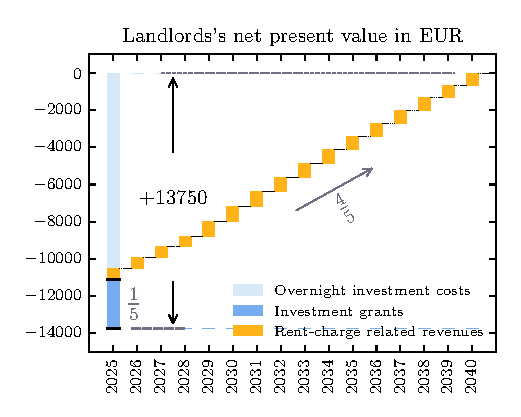
\includegraphics[width=1\linewidth]{figures/3_Methodology/Validate-Landlord.eps}
		\subcaption{Development of landlord's net present value}
		\label{fig:landlord}
	\end{subfigure}
	\begin{subfigure}[c]{0.5\textwidth}
		\centering
		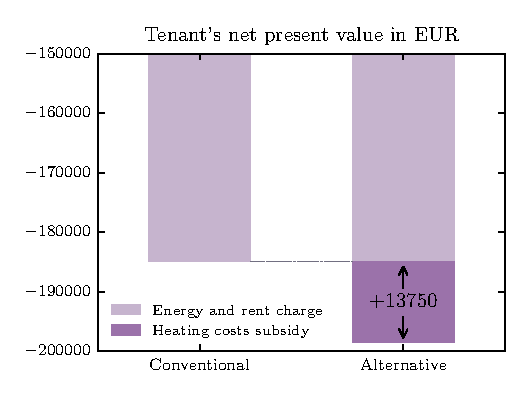
\includegraphics[width=1\linewidth]{figures/3_Methodology/Validate-Tenant.eps}
		\subcaption{Comparison of tenant's net present value}
		\label{fig:tenant}
	\end{subfigure}
	\caption{Landlord's and tenant's net present value and equal financial support. The landlord reaches a net present value equal to zero in 2040 resulting from an investment grant and rent-charge related revenues. The tenant's net present value remains constant compared to the conventional heating system resulting from heating costs subsidy payments.}
	\label{val:npv}
\end{figure}

Both agents receive equal financial support with a total of \SI{13750}{EUR}. One finfth of the landlord's support is paid as an investment grant and four-fifths as rent-charge related revenues. The tenant receives a heating costs subsidy. The level of financial support results exactly in (i) a landlord's net present value equal to zero within the time horizon of 15 years (see Figure \ref{fig:landlord}) and (ii) a constant remaining net present value of tenant compared to the conventional (existing) heating system (including the initial rent charge) (see Figure \ref{fig:tenant}). 

\subsection{Open-source programming environment and data format}\label{met:os}
The developed optimization model is implemented in Python using the modeling framework Pyomo \cite{hart2017optimization}. It is solved with the solver Gurobi version 9.0.3. We use for data analysis the common data format template developed by the Integrated Assessment Modeling Consortium (IAMC) using the open-source Python package pyam \cite{huppmann2021pyam}. Note that all materials used in this study are disclosed as part of the publication at GitHub \footnote{https://github.com/sebastianzwickl}. We refer to the repository for the codebase, data collection, and further information. 